\documentclass[landscape,final,paperwidth=60in,paperheight=41.5in,fontscale=0.285]{baposter}
%\usepackage{calc,array}
\usepackage{graphicx} % Required for including images
\usepackage{amsmath}  % For typesetting math
\usepackage{amssymb}  % Adds new symbols to be used in math mode
\usepackage{relsize}  % Chagnge size of text /smaller, /larger
\usepackage{multirow} % Allows table cells to span more than one row of the table
\usepackage{rotating} % Rotate figures and tables
\usepackage{bm}       % Allows a math expression to be bold
\usepackage{url}      % Allows email address and websites
\usepackage{gensymb}  % Allows degree symbol

\usepackage{float}
\usepackage{caption} % Required for specifying captions to tables and figures
\usepackage{wrapfig} % Wrap text around figure
\usepackage[export]{adjustbox}

\captionsetup[figure]{font=Large,skip=0pt,labelformat=empty,justification=raggedright,singlelinecheck=false}

\usepackage{multicol} % Required for multiple columns

\usepackage[utf8]{inputenc} %Required for IEEE reference style
\newcommand{\BIBdecl}{\setlength{\itemsep}{-0.25 em}} %Removes line space between references

% Fonts
%\usepackage{times}
%\usepackage{helvet}
%\usepackage{bookman}
\usepackage{palatino}

%\newcommand{\captionfont}{\footnotesize}

\graphicspath{{images/}{../images/}}
%\usetikzlibrary{calc}

\newcommand{\SET}[1]  {\ensuremath{\mathcal{#1}}}
\newcommand{\MAT}[1]  {\ensuremath{\boldsymbol{#1}}}
\newcommand{\VEC}[1]  {\ensuremath{\boldsymbol{#1}}}
\newcommand{\Video}{\SET{V}}
\newcommand{\video}{\VEC{f}}
\newcommand{\track}{x}
\newcommand{\Track}{\SET T}
\newcommand{\LMs}{\SET L}
\newcommand{\lm}{l}
\newcommand{\PosE}{\SET P}
\newcommand{\posE}{\VEC p}
\newcommand{\negE}{\VEC n}
\newcommand{\NegE}{\SET N}
\newcommand{\Occluded}{\SET O}
\newcommand{\occluded}{o}

%%%%%%%%%%%%%%%%%%%%%%%%%%%%%%%%%%%%%%%%%%%%%%%%%%%%%%%%%%%%%%%%%%%%%%%%%%%%%%%%
% Multicol Settings
%%%%%%%%%%%%%%%%%%%%%%%%%%%%%%%%%%%%%%%%%%%%%%%%%%%%%%%%%%%%%%%%%%%%%%%%%%%%%%%%
\setlength{\columnsep}{1.5em}
\setlength{\columnseprule}{0mm}
%%%%%%%%%%%%%%%%%%%%%%%%%%%%%%%%%%%%%%%%%%%%%%%%%%%%%%%%%%%%%%%%%%%%%%%%%%%%%%%%
% Save space in lists. Use this after the opening of the list
%%%%%%%%%%%%%%%%%%%%%%%%%%%%%%%%%%%%%%%%%%%%%%%%%%%%%%%%%%%%%%%%%%%%%%%%%%%%%%%%
\newcommand{\compresslist}{%
\setlength{\itemsep}{1pt}%
\setlength{\parskip}{0pt}%
\setlength{\parsep}{0pt}%
}
%%%%%%%%%%%%%%%%%%%%%%%%%%%%%%%%%%%%%%%%%%%%%%%%%%%%%%%%%%%%%%%%%%%%%%%%%%%%%%
%%% Begin of Document
%%%%%%%%%%%%%%%%%%%%%%%%%%%%%%%%%%%%%%%%%%%%%%%%%%%%%%%%%%%%%%%%%%%%%%%%%%%%%%

\begin{document}

%%%%%%%%%%%%%%%%%%%%%%%%%%%%%%%%%%%%%%%%%%%%%%%%%%%%%%%%%%%%%%%%%%%%%%%%%%%%%%
%%% Here starts the poster
%%%---------------------------------------------------------------------------
%%% Format it to your taste with the options
%%%%%%%%%%%%%%%%%%%%%%%%%%%%%%%%%%%%%%%%%%%%%%%%%%%%%%%%%%%%%%%%%%%%%%%%%%%%%%
% Define some colors

%\definecolor{lightblue}{cmyk}{0.83,0.24,0,0.12}
\definecolor{lightblue}{rgb}{0.145,0.6666,1}

%\newtcolorbox{demobox}[1][]{colback=white,colframe=lightblue,width=0.33\linewidth,nobeforeafter,box align=top,before=\noindent,#1}

%%
\begin{poster}%
  % Poster Options
  {
  % Show grid to help with alignment
  grid=false,
  % Column spacing
  colspacing=1em,
  % Color style
  bgColorOne=white,
  bgColorTwo=white,
  borderColor=lightblue,
  headerColorOne=black,
  headerColorTwo=lightblue,
  headerFontColor=white,
  boxColorOne=white,
  boxColorTwo=lightblue,
  % Format of textbox
  textborder=roundedleft,
  % Format of text header
  eyecatcher=true,
  headerborder=closed,
  headerheight=0.12\textheight,
  columns=4, %default=4 for landscape posters maximum columns=6
%  textfont=\sc, An example of changing the text font
  headershape=roundedright,
  headershade=shadelr,
  headerfont=\Large\bf\textsc, %Sans Serif
  textfont={\setlength{\parindent}{1.5em}},
  boxshade=plain,
%  background=shade-tb,
  background=plain,
  linewidth=2pt
  }
  % University logo
  {
\includegraphics[height=6em]{img/penn_state_cla_logo_new_210-89.jpg}}
  % Title
  {\bf{School-age children perceive fast radial optic flow in noise\\more accurately than slow linear flow} \vspace{0.2em}}
  % Authors
  {Rick O. Gilmore \emph{(rogilmore@psu.edu)}, Andrea R. Seisler, Michelle A. Shade, \& Michael J. O'Neill\\ \vspace{0.2em}
  SRCD 2017 -- Poster xxxxx}
  % Databrary Logo
 {
\includegraphics[height=4em]{img/databrary.png}}

%%%%%%%%%%%%%%%%%%%%%%%%%%%%%%%%%%%%%%%%%%%%%%%%%%%%%%%%%%%%%%%%%%%%%%%%%%%%%%
%%% Now define the boxes that make up the poster
%%%---------------------------------------------------------------------------
%%% Each box has a name and can be placed absolutely or relatively.
%%% The only inconvenience is that you can only specify a relative position
%%% towards an already declared box. So if you have a box attached to the
%%% bottom, one to the top and a third one which should be in between, you
%%% have to specify the top and bottom boxes before you specify the middle
%%% box.
%%%%%%%%%%%%%%%%%%%%%%%%%%%%%%%%%%%%%%%%%%%%%%%%%%%%%%%%%%%%
%
%%%%%%%%%%%%%%%%%%%%%%%%%%%%%%%%%%%%%%%%%%%%%%%%%%%%%%%%%%%%%%%%%%%%%%%%%%%%%%
\headerbox{Motivation}{name=abstract,column=0,span = 1,row=0}
%%%%%%%%%%%%%%%%%%%%%%%%%%%%%%%%%%%%%%%%%%%%%%%%%%%%%%%%%%%%%%%%%%%%%%%%%%%%%%
    {
      Optic flow evokes different cortical activation patterns across the scalp depending on the pattern of flow (radial vs. linear) and speed. These effects are seen both in adults \cite{Fesi2014-pi} and children \cite{Gilmore2016-sd}. This study examined whether the detection of optic flow in child observers varies by pattern and speed in similar ways to adults \cite{Adamiak2015-lo},\cite{Adamiak2015-tw}, and the extent to which behavioral detection accords with patterns of brain activation.
    }
%%%%%%%%%%%%%%%%%%%%%%%%%%%%%%%%%%%%%%%%%%%%%%%%%%%%%%%%%%%%%%%%%%%%%%%%%%%%%%
\headerbox{Method}{name=method,column=0,span = 1,below=abstract}
%%%%%%%%%%%%%%%%%%%%%%%%%%%%%%%%%%%%%%%%%%%%%%%%%%%%%%%%%%%%%%%%%%%%%%%%%%%%%%
    {
Child observers (n=31; 5.2-8.6 years, \emph{M}=6.7, 19 female) participated for \$10 in compensation. Observers judged which of two side-by-side optic flow displays contained coherent motion. Each run contained 5 blocks of 16 trials in which one display depicted random (0\% coherent) motion while the other depicted radial or linear motion at one of four fixed coherence levels in one of two coherence level profiles (20, 40, 60, 80\%) or (15, 30, 45, 60\%). Observers fixated centrally and judged which side contained coherent motion, indicating the choice by pointing to the monitor. The choice was entered by the experimenter via keypress. Within a single run, speed was either 2 or 8 deg/s. Four runs were collected per participant in a single visit lasting approximately 1 hour. Participants were given the option to take a break half way through the experiment. 
\par
We analyzed the proportion of correct responses and response times using generalized linear mixed effects modeling in R.
\par
    }
%%%%%%%%%%%%%%%%%%%%%%%%%%%%%%%%%%%%%%%%%%%%%%%%%%%%%%%%%%%%%%%%%%%%%%%%%%%%%%
\headerbox{Displays}{name=displays,column=3, span=1, row=0}
%%%%%%%%%%%%%%%%%%%%%%%%%%%%%%%%%%%%%%%%%%%%%%%%%%%%%%%%%%%%%%%%%%%%%%%%%%%%%%
    {
Two side-by-side, time varying (1.2 Hz coherent/incoherent cycle) annular-shaped (18\degree outer/5\degree inner diameter) optic flow displays were presented at a viewing distance of 60 cm. Optic flow was generated by random dot kinematograms with white dots (110 cd/m, 7 amin) presented on a black background. In each trial, one display depicted random (0\% coherent) motion while the other depicted radial or linear motion at one of four fixed coherence levels in one of two coherence level profiles (20, 40, 60, 80\%) or (15, 30, 45, 60\%).
%\vspace{-1.3em}    %remove extra space at top of box
%\begin{wrapfigure}{R}{5cm}
\centering
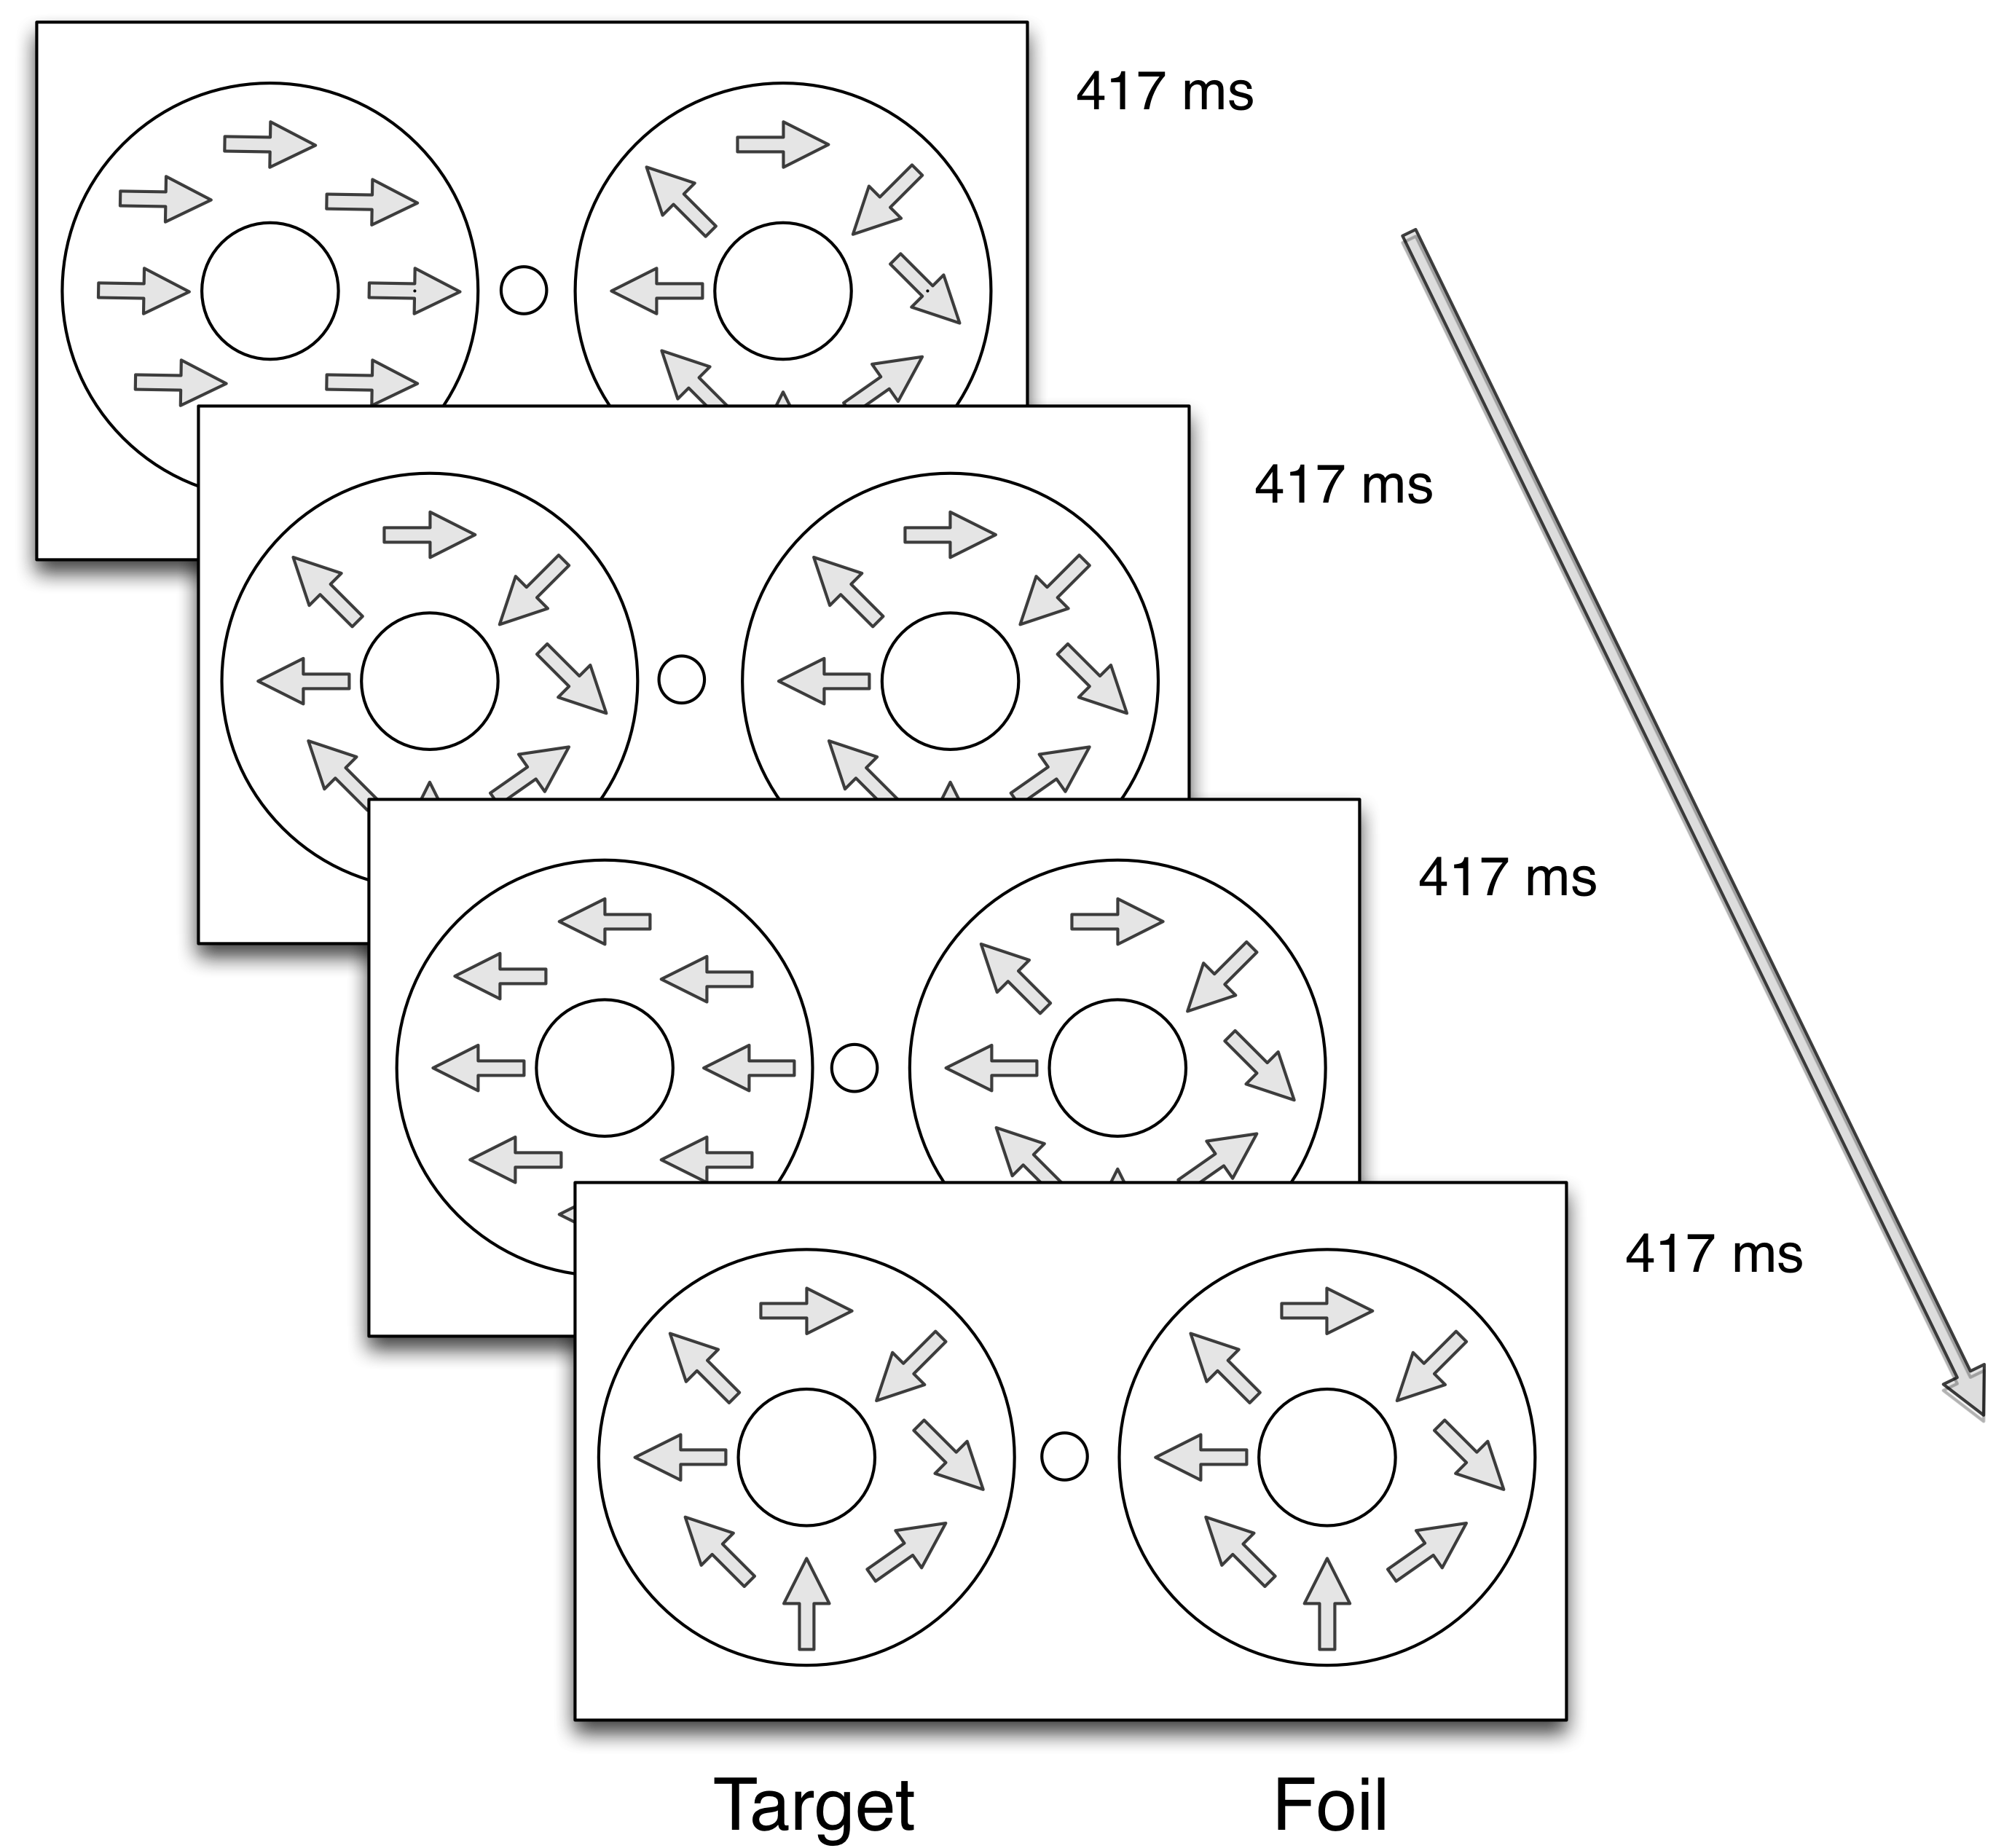
\includegraphics[scale=0.4]{img/optic-flow-psychophysics-display.png}
%\par
%\end{wrapfigure}
    }
%%%%%%%%%%%%%%%%%%%%%%%%%%%%%%%%%%%%%%%%%%%%%%%%%%%%%%%%%%%%%%%%%%%%%%%%%%%%%%
\headerbox{Results}{name=results,column=1,span=2,row=0}
%%%%%%%%%%%%%%%%%%%%%%%%%%%%%%%%%%%%%%%%%%%%%%%%%%%%%%%%%%%%%%%%%%%%%%%%%%%%%%
    {
Coherence \(\chi^{2}(1)=??, p<.??\), pattern type \(\chi^{2}(1)=??, p<.??\), coherence by pattern type \(\chi^{2}(1)=??, p<.??\), and speed \(\chi^{2}(1)=??, p<.??\) remained in the final model for proportion correct judgments.

As coherence increased from 15 to 80\%, accuracy to detect radial flows increased from .x to .x and for translational flows from .x to .x.

We found comparable effects for reaction time.
 
As predicted, the proportion of correct judgments increased and the response times of correct judgements declined with increasing motion coherence. Fast optic flow patterns were perceived more reliably than slow, and radial patterns were perceived more reliably than linear patterns. Taken together the results suggest that school-age children's abilities to detect radial and linear optic flow patterns in noise are somewhat less precise than adults', although their biases toward faster radial patterns are adult-like.

\begin{center}
  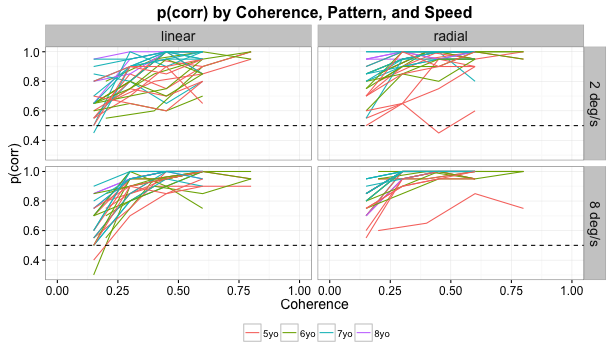
\includegraphics[scale=0.7,valign=t]{img/p-corr-plot-1.png}

  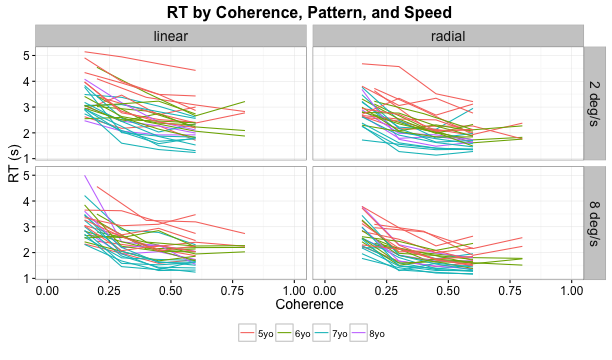
\includegraphics[scale=0.7,valign=t]{img/rt-plot-1.png}
\end{center}
}
%%%%%%%%%%%%%%%%%%%%%%%%%%%%%%%%%%%%%%%%%%%%%%%%%%%%%%%%%%%%%%%%%%%%%%%%%%%%%%
   \headerbox{Data Sharing}{name=sharing, column=3, below=displays}
%%%%%%%%%%%%%%%%%%%%%%%%%%%%%%%%%%%%%%%%%%%%%%%%%%%%%%%%%%%%%%%%%%%%%%%%%%%%%%%
    {
       Movies of the displays, metadata about the participants, and raw data files are available at: \url{http://databrary.org/volume/218}.
     }
%%%%%%%%%%%%%%%%%%%%%%%%%%%%%%%%%%%%%%%%%%%%%%%%%%%%%%%%%%%%%%%%%%%%%%%%%%%%%%
  \headerbox{Acknowledgements}{name=thanks, column=3, below=sharing}
%%%%%%%%%%%%%%%%%%%%%%%%%%%%%%%%%%%%%%%%%%%%%%%%%%%%%%%%%%%%%%%%%%%%%%%%%%%%%%
    {
    \smaller
      This material is based upon work supported by the National Science Foundation under Grant Number BCS-1147440. Any opinions, findings, and conclusions or recommendations expressed in this material are those of the author(s) and do not necessarily reflect the views of the National Science Foundation.
    }
%%%%%%%%%%%%%%%%%%%%%%%%%%%%%%%%%%%%%%%%%%%%%%%%%%%%%%%%%%%%%%%%%%%%%%%%%%%%%%
 \headerbox{References}{name=references, column=3, below=thanks}
%%%%%%%%%%%%%%%%%%%%%%%%%%%%%%%%%%%%%%%%%%%%%%%%%%%%%%%%%%%%%%%%%%%%%%%%%%%%%%
  {
          \tiny
  %For use with external .bib file
          \renewcommand{\refname}{\vspace{-0.5em}} % removes "References" canned text.
          \bibliographystyle{IEEEtran}
          \bibliography{IEEEabrv,poster_landscape}

}
\end{poster}%
%
\end{document}
